Authors: \href{http://peeragogy.org/resources/meet-the-team/}{The
Peeragogy Team}

\begin{quote}
Although a grounding in learning theory helps inform peer learning
projects, Peeragogy, at its core, comes to life in applied practice. For
a successful outcome, take a look at these best practices, patterns, and
use cases (also called \emph{case studies} or \emph{examples}). Patterns
and use cases that co-facilitators and participants identify as the
project unfolds can serve the next peeragogical enterprise as well.

\end{quote}
\subsection{}

\subsection{What is a pattern?}

A pattern is anything that has a repeated effect. In the context of
peeragogy, the practice is to repeat processes and interactions that
advance the learning mission. Frequent occurrences that are not
desirable are called anti-patterns!

\begin{quote}
\textbf{Christopher Alexander}: ``Each pattern describes a problems
which occurs over and over again in our environment, and then describes
the core of the solution to that problem, in a way that you can use this
solution a million times over, without ever doing it the same way
twice.'' {[}1{]}

\end{quote}
Patterns provide a framework that can be applied to similar issues but
may be metaphorically solved in different ways, sometimes in real world
or face to face events and other times in digital space / applications.

\begin{quote}
\textbf{Christopher Alexander}: ``Can we do better? Does all this talk
help to make better buildings? {[}\ldots{}{]} What is the Chartres of
programming? What task is at a high enough level to inspire people
writing programs, to reach for the stars?'' {[}2{]}

\end{quote}
Note: the notion of the analog (such as a plaza) could become a digital
metaphor for a group chat or Google+ Hangout -- a group meeting space /
agora. Indeed the working title for Google Communities was ``piazza!''

\subsection{Patterns of peeragogy}

Here is our index of the patterns we've found so far (described in more
detail after the jump):

\begin{itemize}
\item
  \href{http://peeragogy.org/patterns/wrapper/}{Wrapper} - Front end
  appearance to participants. Consolidate and summarize.
\item
  \href{http://peeragogy.org/patterns/discerning-a-pattern/}{Discerning
  a pattern} - Found a pattern? Give it a title and example.
\item
  \href{http://peeragogy.org/patterns/polling-for-ideas/}{Polling for
  ideas} - Invite brainstorming, collecting ideas, questions, and
  solutions.
\item
  \href{http://peeragogy.org/patterns/creating-a-guide/}{Creating a
  guide} - Overviews expose the lay of the land. Collecting content and
  stories.
\item
  \href{http://peeragogy.org/patterns/newcomer/}{Newcomer} - Create a
  guide for ``beginner's mind'' and help avoid need to introduce new
  members each ``meeting.''
\item
  \href{http://peeragogy.org/patterns/roadmap/}{Roadmap} - Plans for
  future work, direction towards a goal, dynamic
\item
  \href{http://peeragogy.org/patterns/roles/}{Roles} - Specialize and
  mix it up. Play to participants strengths and skills.
\item
  \href{http://peeragogy.org/focusing-on-a-specific-project/}{Project
  focus} - Lightbulb moment: Most specific projects involve learning!
\item
  \href{http://peeragogy.org/patterns/carrying-capacity/}{Carrying
  capacity} - Know your limits, find ways to get other people involved.
\item
  \href{http://peeragogy.org/patterns/heartbeat/}{Heartbeat} - The
  ``heartbeat'' of the group keeps energy flowing.
\item
  \href{http://peeragogy.org/patterns/moderation/}{Moderation} - When
  leaders step back, dynamics can improve; moderator serves as champion
  and editor.
\item
  \href{http://peeragogy.org/patterns/praxis-vs-poeisis/}{Use or make?}
  - Repurposing, tinkering, or creating from scratch?
\item
  \href{http://peeragogy.org/reiterate/}{Reiterate} - Periodically
  review and revise above actions as needed
\end{itemize}
\subsection{Anti-patterns for Peeragogy}

And some ``anti-patterns'' (things to avoid):

\begin{itemize}
\item
  \href{http://peeragogy.org/antipatterns/isolation/}{Isolation} - A
  tale of silos, holes, and not-invented-here.
\item
  \href{http://peeragogy.org/antipatterns/magical-thinking/}{Magical
  thinking} - ``One meeting will (not) change everything!''
\item
  \href{http://peeragogy.org/antipatterns/co-learning-messy-with-lurkers/}{Messy
  with Lurkers} - What happens when joining is low-cost and completion
  is low-benefit.
\item
  \href{http://peeragogy.org/antipatterns/misunderstanding-power/}{Misunderstanding
  Power} - The workload is almost never evenly distributed.
\item
  \href{http://peeragogy.org/antipatterns/navel-gazing/}{Navel Gazing} -
  ``I have this really great idea\ldots{}''
\item
  \href{http://peeragogy.org/antipatterns/stasis/}{Stasis} - What's the
  driver behind open source, commons-oriented collaborative projects?
  (Because, let's face it, it doesn't always work.)
\item
  \href{http://peeragogy.org/antipatterns/stuck-at-the-level-of-weak-ties/}{Stuck
  at the level of weak ties} - can we deepen the connection?
\end{itemize}
\subsection{What is a use case?}

A use case describes someone (or something) who uses a given system or
tool to achieve a goal. A use case can include a title, a summary of
the problem, an actor, and a success scenario. Additional features can
be added, such as alternate interactions or choices that lead to a
variation on the result.  The use case considers a given persona (a
characteristic role) in a given situation and shows how they works on
a project/problem and how their process of work is resolved into a
solution or solutions. Some activities do not have a single solution
-- these are often referred to as ``Wicked Problems.'' With detailed
bookkeeping effort, recorded processes can be standardized into use
cases that can then be employed directly or modified to fit the
context of the activity at hand. In short, they are a lot like design
patterns, which they may contain in hidden or explicit form. Use cases
are presented in sidebars and vignettes that appear throughout the
book (like the one below).

\subsection{Pattern language}

Combine patterns and use cases and you start to identify a
\href{http://peeragogy.org/practice/heuristics/pattern-language/}{pattern
language} that can be used immediately, and in future projects. The next
section on \href{http://peeragogy.org/practice/heuristics/}{problem
solving} goes into more detail, but we'll preview the idea here with the
following diagram:

\begin{figure}[htbp]
\centering
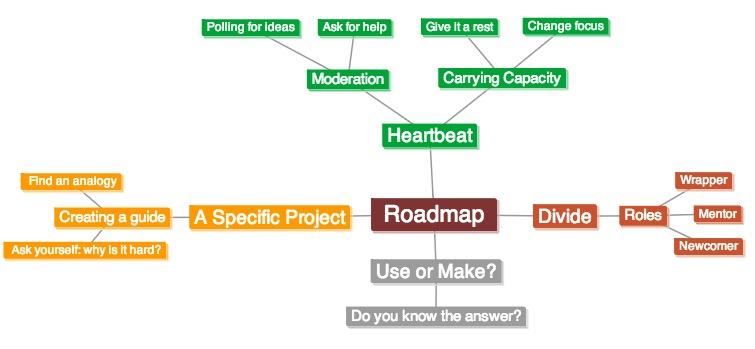
\includegraphics[width=\textwidth]{../pictures/pattern-map1.jpg}
%\caption*{A map of some of the main features of our pattern language}
\end{figure}

The subsequent major sections of this book --
\href{http://peeragogy.org/convene/}{\emph{Convene}},
\href{http://peeragogy.org/organize/}{\emph{Organize}},
\href{http://peeragogy.org/facilitate/}{\emph{Cooperate}} and
\href{http://peeragogy.org/assessment/}{\emph{Assess}} -- represent big
clusters of patterns that are likely to come up time and again in
various projects (do you see the analogy with the four major branches of
the diagram above?). You are of course free to invent your own patterns.
Each project will tend to have it's own design, and it's own unique way
things play out in practice. Here, we present these small but powerful
``starter patterns''.

\begin{quote}
\textbf{Christopher Alexander}: These ideas---patterns---are hardly more
than glimpses of a much deeper level of structure, and is ultimately
within this deeper level of structure, that the origin of life occurs.
\end{quote}
\subsubsection{\textbf{EXAMPLES}}

The above use cases and patterns make the ``story'' abstract -- but how
about some concrete examples of peeragogy in action? Consider:

\begin{itemize}
\item
  \href{http://openhatch.org/}{OpenHatch.org}, ``an open source
  community aiming to help newcomers find their way into free software
  projects.''
\item
  The
  \href{http://campus.ftacademy.org/wiki/index.php/Free\_Technology\_Guild}{Free
  Technology Guild} is a younger project with aspirations similar in
  some ways to those of OpenHatch, but in this case, oriented not just
  to pairing newcomers with mentors, but pairing clients with service
  providers. ``The idea is that we as a group will do useful projects
  for our members or external parties, and on-the-job we mentor and
  learn and get better.'' (Since this is a new project, the
  \href{http://campus.ftacademy.org/community/pg/groups/8500/free-technology-guild-working-group/}{project
  building phase} is itself a nacent example of paragogy.)
\item
  Many more examples on our
  \href{http://peeragogy.org/examples/}{examples} page!
\end{itemize}
\subsubsection{References}

\begin{enumerate}
\item
  Alexander, Christopher, Ishikawa, Sara, and Silverstein, Murray,
  \emph{A Pattern Language: Towns, Buildings, and, Construction}, New
  York: Oxford University Press, 1977.
\item
  Gabriel, Richard P.
  \emph{\href{http://dreamsongs.net/Files/PatternsOfSoftware.pdf}{Patterns
  of Software}}, New York: Oxford University Press, 1996. (Includes a
  forward by Christopher Alexander.)
\end{enumerate}
\subsubsection{Further readings on patterns}

\begin{enumerate}
\item
  \href{http://en.wikipedia.org/wiki/The\_Timeless\_Way\_of\_Building}{The
  Timeless Way of Building}, by Christopher Alexander.
\item
  Article, ``Manifesto 1991'' by Christopher Alexander, Progressive
  Architecture, July 1991, pp. 108--112, provides a brief summary of
  Alexander's ideas in the form of a critique of mainstream
  architecture. Many of the same sorts of critical points would carry
  over to mainstream education. Some highlights are excerpted
  \href{https://plus.google.com/u/0/108598104736826154120/posts/agWYcqPhqSN}{here}.
\item
  \href{http://www.wikipatterns.com/display/wikipatterns/About}{Wikipatterns}
\item
  \href{http://www.patternlanguage.com/archive/ieee/ieeetext.htm}{The
  Origins of Pattern Theory, the Future of the Theory, And The
  Generation of a Living World}, Christopher Alexander's talk at the
  1996 ACM Conference on Object-Oriented Programs, Systems, Languages
  and Applications (OOPSLA)
\end{enumerate}
\subsubsection{Other related work}

\begin{enumerate}
\item
  \href{http://www.cluetrain.com}{Cluetrain Manifesto} (the
  \href{http://www.cluetrain.com/book/index.html}{First edition} is
  available for free)
\item
  \href{http://www.kk.org/newrules/contents.php}{New Rules for the New
  Economy}\href{http://www.kk.org/newrules/contents.php}{(you can
  also}\href{http://www.kk.org/newrules/contents.php}{read the book
  online})
\end{enumerate}
